\begin{figure}[ht!]
\centering
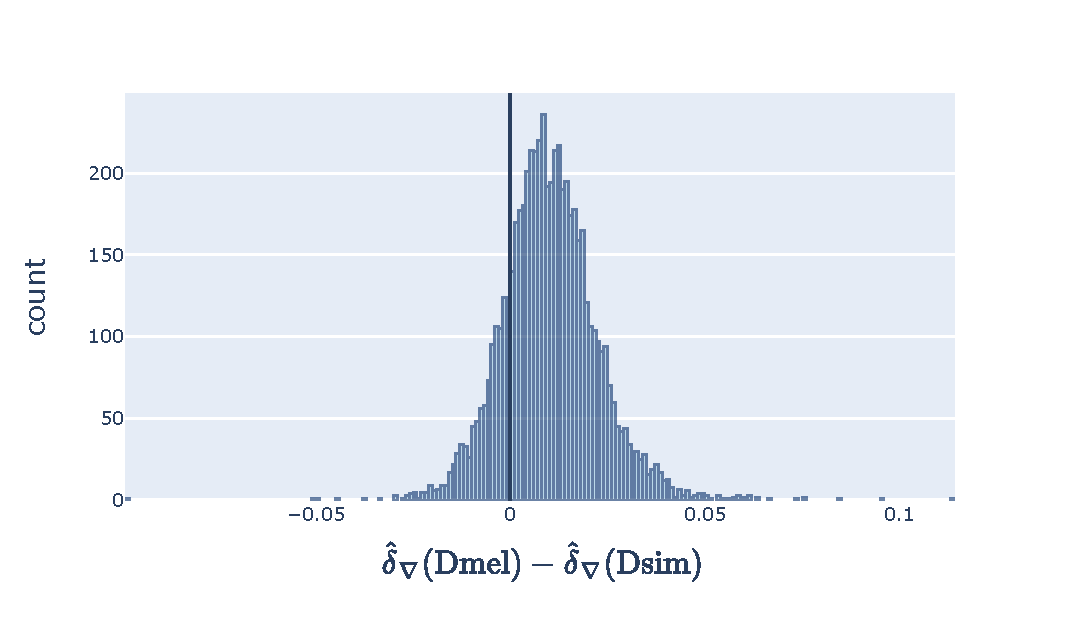
\includegraphics[width=	\textwidth]{figures/plots/drosophila/d-conv-diff.pdf}
\caption{\textbf{The magnitude of mutation disequilibrium is higher in \textit{D. melanogaster} than in \textit{D. simulans}}. Each data point in the distribution is the difference between $\hat\delta_\nabla$ for a gene in \textit{D. melanogaster} and in its ortholog in \textit{D. simulans}. If the magnitude of $\hat\delta_\nabla$ in both species was the same, the distribution would be centred on the vertical line on zero. 82\% of genes had a higher $\delta_\nabla$ estimate in \textit{D. melanogaster}. Data included from $\sim 5,900$ CDS alignments of \textit{D. melanogaster}, \textit{D. simulans} and \textit{D. yakubra}. The CDS sequence of the gene is third codon position only.}
\label{fig:drosophila_d-conv-diff}
\end{figure}
